
\documentclass[a4paper, 10pt, twoside]{article}

\usepackage[top=1in, bottom=1in, left=1in, right=1in]{geometry}
\usepackage[utf8]{inputenc}
\usepackage[spanish, es-ucroman, es-noquoting]{babel}
\usepackage{setspace}
\usepackage{fancyhdr}
\usepackage{lastpage}
\usepackage{amsmath}
\usepackage{amsfonts}
\usepackage{amsthm}
\usepackage{verbatim}
\usepackage{fancyvrb}
\usepackage{graphicx}
\usepackage{float}
\usepackage{enumitem} % Provee macro \setlist
\usepackage{tabularx}
\usepackage{multirow}
\usepackage{hyperref}
\usepackage{xspace}
\usepackage{ulem} % Provee macro \uwave
\usepackage[toc, page]{appendix}


%%%%%%%%%% Constantes - Inicio %%%%%%%%%%
\newcommand{\titulo}{Trabajo Práctico 1}
\newcommand{\materia}{Bases de Datos}
\newcommand{\integrantes}{Russo · Russo · Russo · Russo}
\newcommand{\cuatrimestre}{Primer Cuatrimestre de 2016}
%%%%%%%%%% Constantes - Fin %%%%%%%%%%


%%%%%%%%%% Configuración de Fancyhdr - Inicio %%%%%%%%%%
\pagestyle{fancy}
\thispagestyle{fancy}
\lhead{\titulo · \materia}
\rhead{\integrantes}
\renewcommand{\footrulewidth}{0.4pt}
\cfoot{\thepage /\pageref{LastPage}}

\fancypagestyle{caratula} {
   \fancyhf{}
   \cfoot{\thepage /\pageref{LastPage}}
   \renewcommand{\headrulewidth}{0pt}
   \renewcommand{\footrulewidth}{0pt}
}
%%%%%%%%%% Configuración de Fancyhdr - Fin %%%%%%%%%%


%%%%%%%%%% Miscelánea - Inicio %%%%%%%%%%
% Evita que el documento se estire verticalmente para ocupar el espacio vacío
% en cada página.
\raggedbottom

% Separación entre párrafos.
\setlength{\parskip}{0.5em}

% Separación entre elementos de listas.
\setlist{itemsep=0.5em}

% Asigna la traducción de la palabra 'Appendices'.
\renewcommand{\appendixtocname}{Apéndices}
\renewcommand{\appendixpagename}{Apéndices}
%%%%%%%%%% Miscelánea - Fin %%%%%%%%%%


%%%%%%%%%% Macros para el modelo relacional - Inicio %%%%%%%%%%
\newcommand{\relacion}[3]{
  \noindent
  \textbf{#1}(\ignorespaces#2\unskip) \\
  #3
  \vspace{0.5em}
}
\newcommand{\pk}[1]{%
  \underline{#1}%
}
\newcommand{\fk}[1]{%
  \uwave{#1}%
}
\newcommand{\pkfk}[1]{%
  \pk{\fk{#1}}%
}
\newcommand{\clavespkck}[1]{
  PK = CK = \{#1\}
}
\newcommand{\clavespkckfk}[1]{
  PK = CK = FK = \{#1\}
}
\newcommand{\clavesfk}[1]{
  FK = \{#1\}
}
%%%%%%%%%% Macros para el modelo relacional - Fin %%%%%%%%%%

\begin{document}


%%%%%%%%%%%%%%%%%%%%%%%%%%%%%%%%%%%%%%%%%%%%%%%%%%%%%%%%%%%%%%%%%%%%%%%%%%%%%%%
%% Carátula                                                                  %%
%%%%%%%%%%%%%%%%%%%%%%%%%%%%%%%%%%%%%%%%%%%%%%%%%%%%%%%%%%%%%%%%%%%%%%%%%%%%%%%


\thispagestyle{caratula}

\begin{center}


\includegraphics[height=2cm]{DC.png} 
\hfill

\includegraphics[height=2cm]{UBA.jpg} 

\vspace{2cm}

Departamento de Computación,\\
Facultad de Ciencias Exactas y Naturales,\\
Universidad de Buenos Aires

\vspace{4cm}

\begin{Huge}
\titulo
\end{Huge}

\vspace{0.5cm}

\begin{Large}
\materia
\end{Large}

\vspace{1cm}

\cuatrimestre

\vspace{4cm}

\begin{tabular}{|c|c|c|}
\hline
Apellido y Nombre & LU & E-mail\\
\hline
Russo, Christian  & 679/10 & christian.russo8@gmail.com\\
Russo, Christian  & 679/10 & christian.russo8@gmail.com\\
Russo, Christian  & 679/10 & christian.russo8@gmail.com\\
Russo, Christian  & 679/10 & christian.russo8@gmail.com\\
\hline
\end{tabular}

\end{center}

\newpage


%%%%%%%%%%%%%%%%%%%%%%%%%%%%%%%%%%%%%%%%%%%%%%%%%%%%%%%%%%%%%%%%%%%%%%%%%%%%%%%
%% Introducción                                                              %%
%%%%%%%%%%%%%%%%%%%%%%%%%%%%%%%%%%%%%%%%%%%%%%%%%%%%%%%%%%%%%%%%%%%%%%%%%%%%%%%


\section{Introducción}

Presentaremos una soluci\'on para el problema de un \textbf{Mercado Virtual} tomando como gu\'ia el \textbf{Khan El-Khalili} ubicado en El Cairo, Egipto. El problema en cuesti\'on contempla una serie de restricciones sobre como se realizan la combra y venta de productos por internet. Cada publicacion puede tener distintos tipos y ser de distintas formas, haciendo que esto impacte en la facturacion del usuario que publica. Por otro lado se cuenta con un sistema de comentarios y calificaciones.

Utilizaremos las herramientas vistas en la materia, el modelado basado en el Diagrama de Entidad Relaci?on, su MR resultante y la base de datos final que presentaremos en MySQL.

%%%%%%%%%%%%%%%%%%%%%%%%%%%%%%%%%%%%%%%%%%%%%%%%%%%%%%%%%%%%%%%%%%%%%%%%%%%%%%%
%% Diagrama de Entidad Relación                                              %%
%%%%%%%%%%%%%%%%%%%%%%%%%%%%%%%%%%%%%%%%%%%%%%%%%%%%%%%%%%%%%%%%%%%%%%%%%%%%%%%


\section{Diagrama de Entidad Relación}

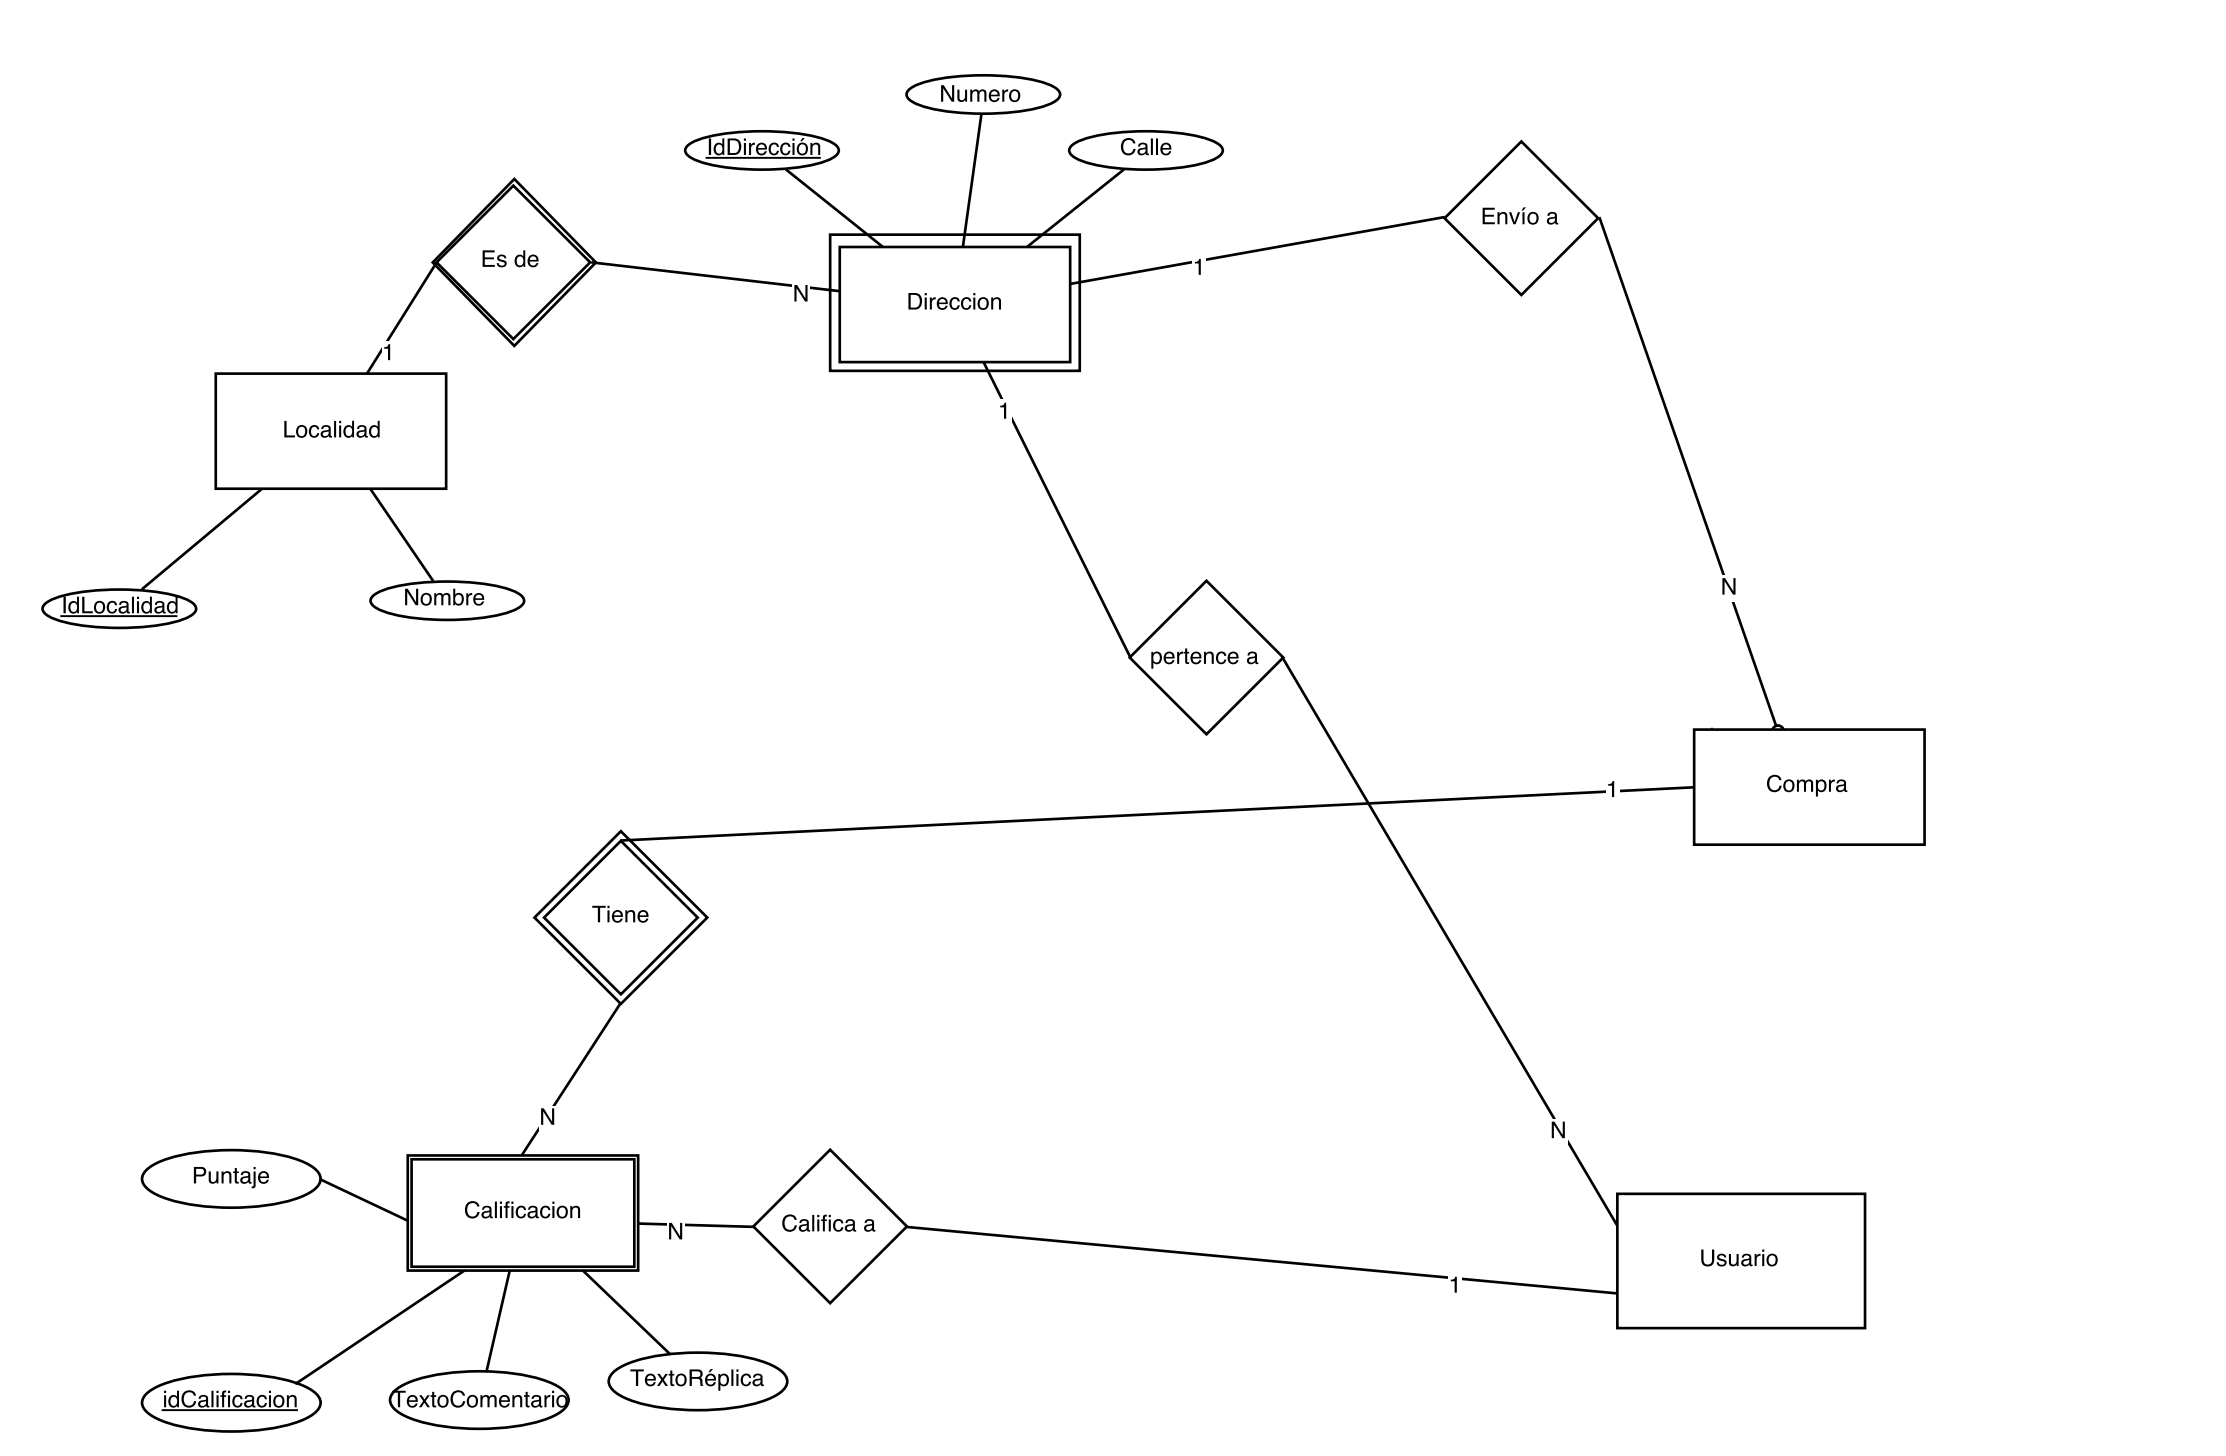
\includegraphics[width=20cm, height=12cm]{der1}
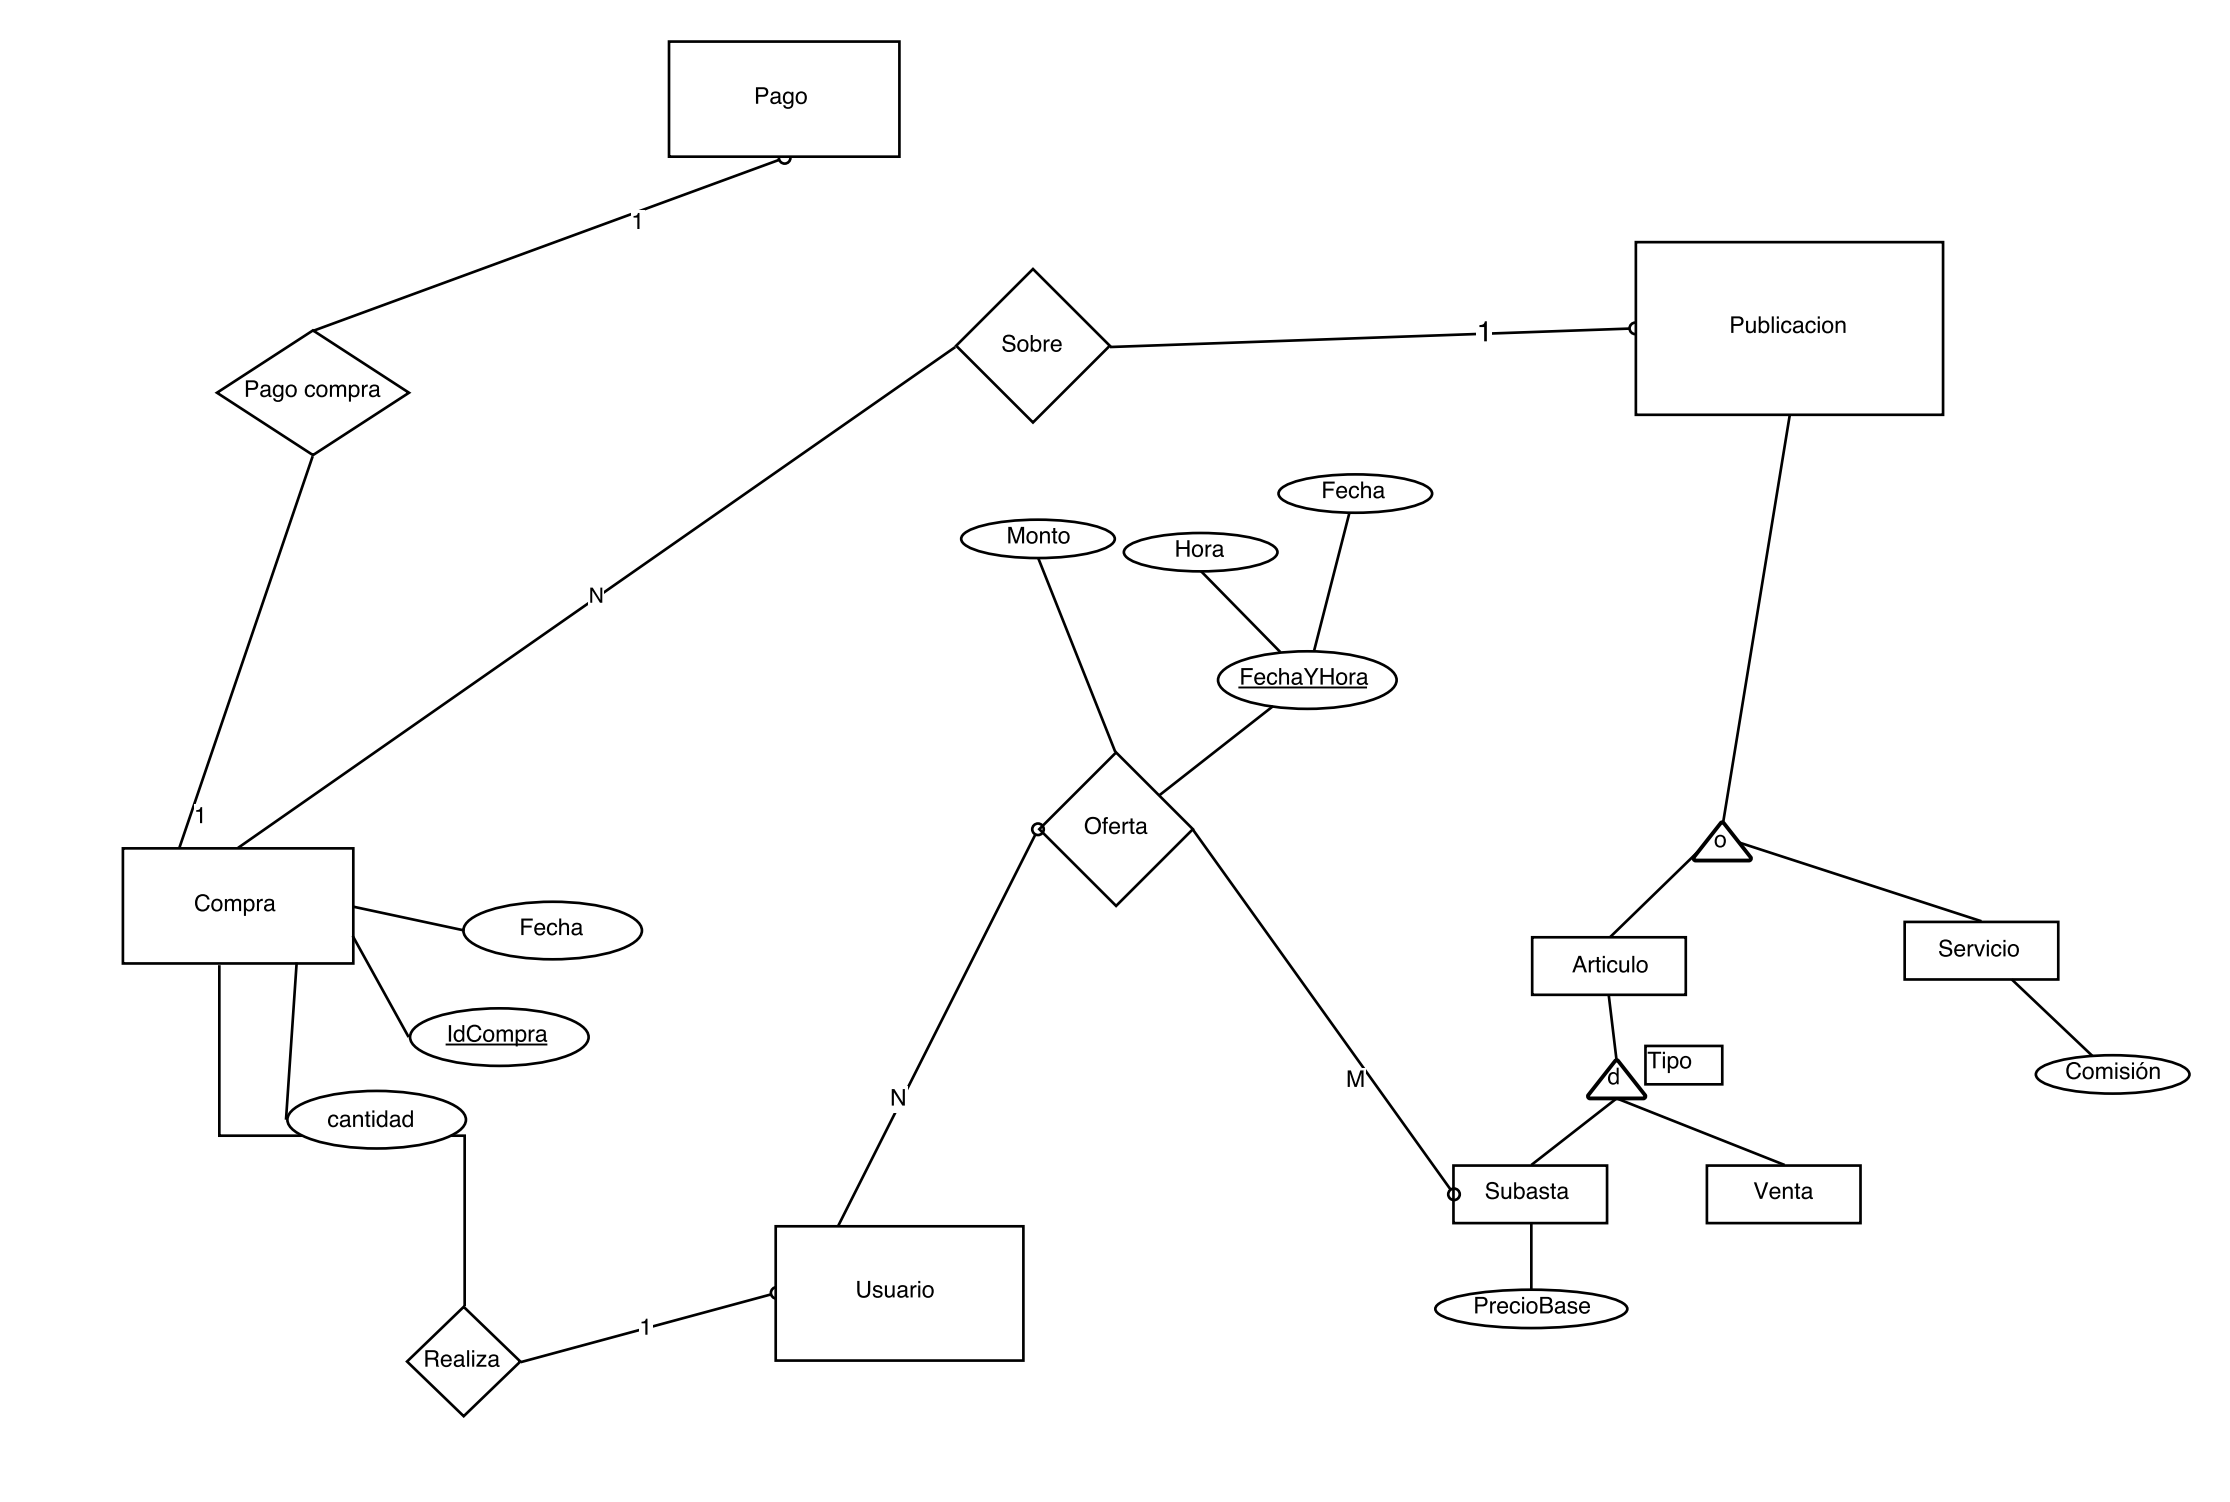
\includegraphics[width=18cm, height=12cm]{der2}
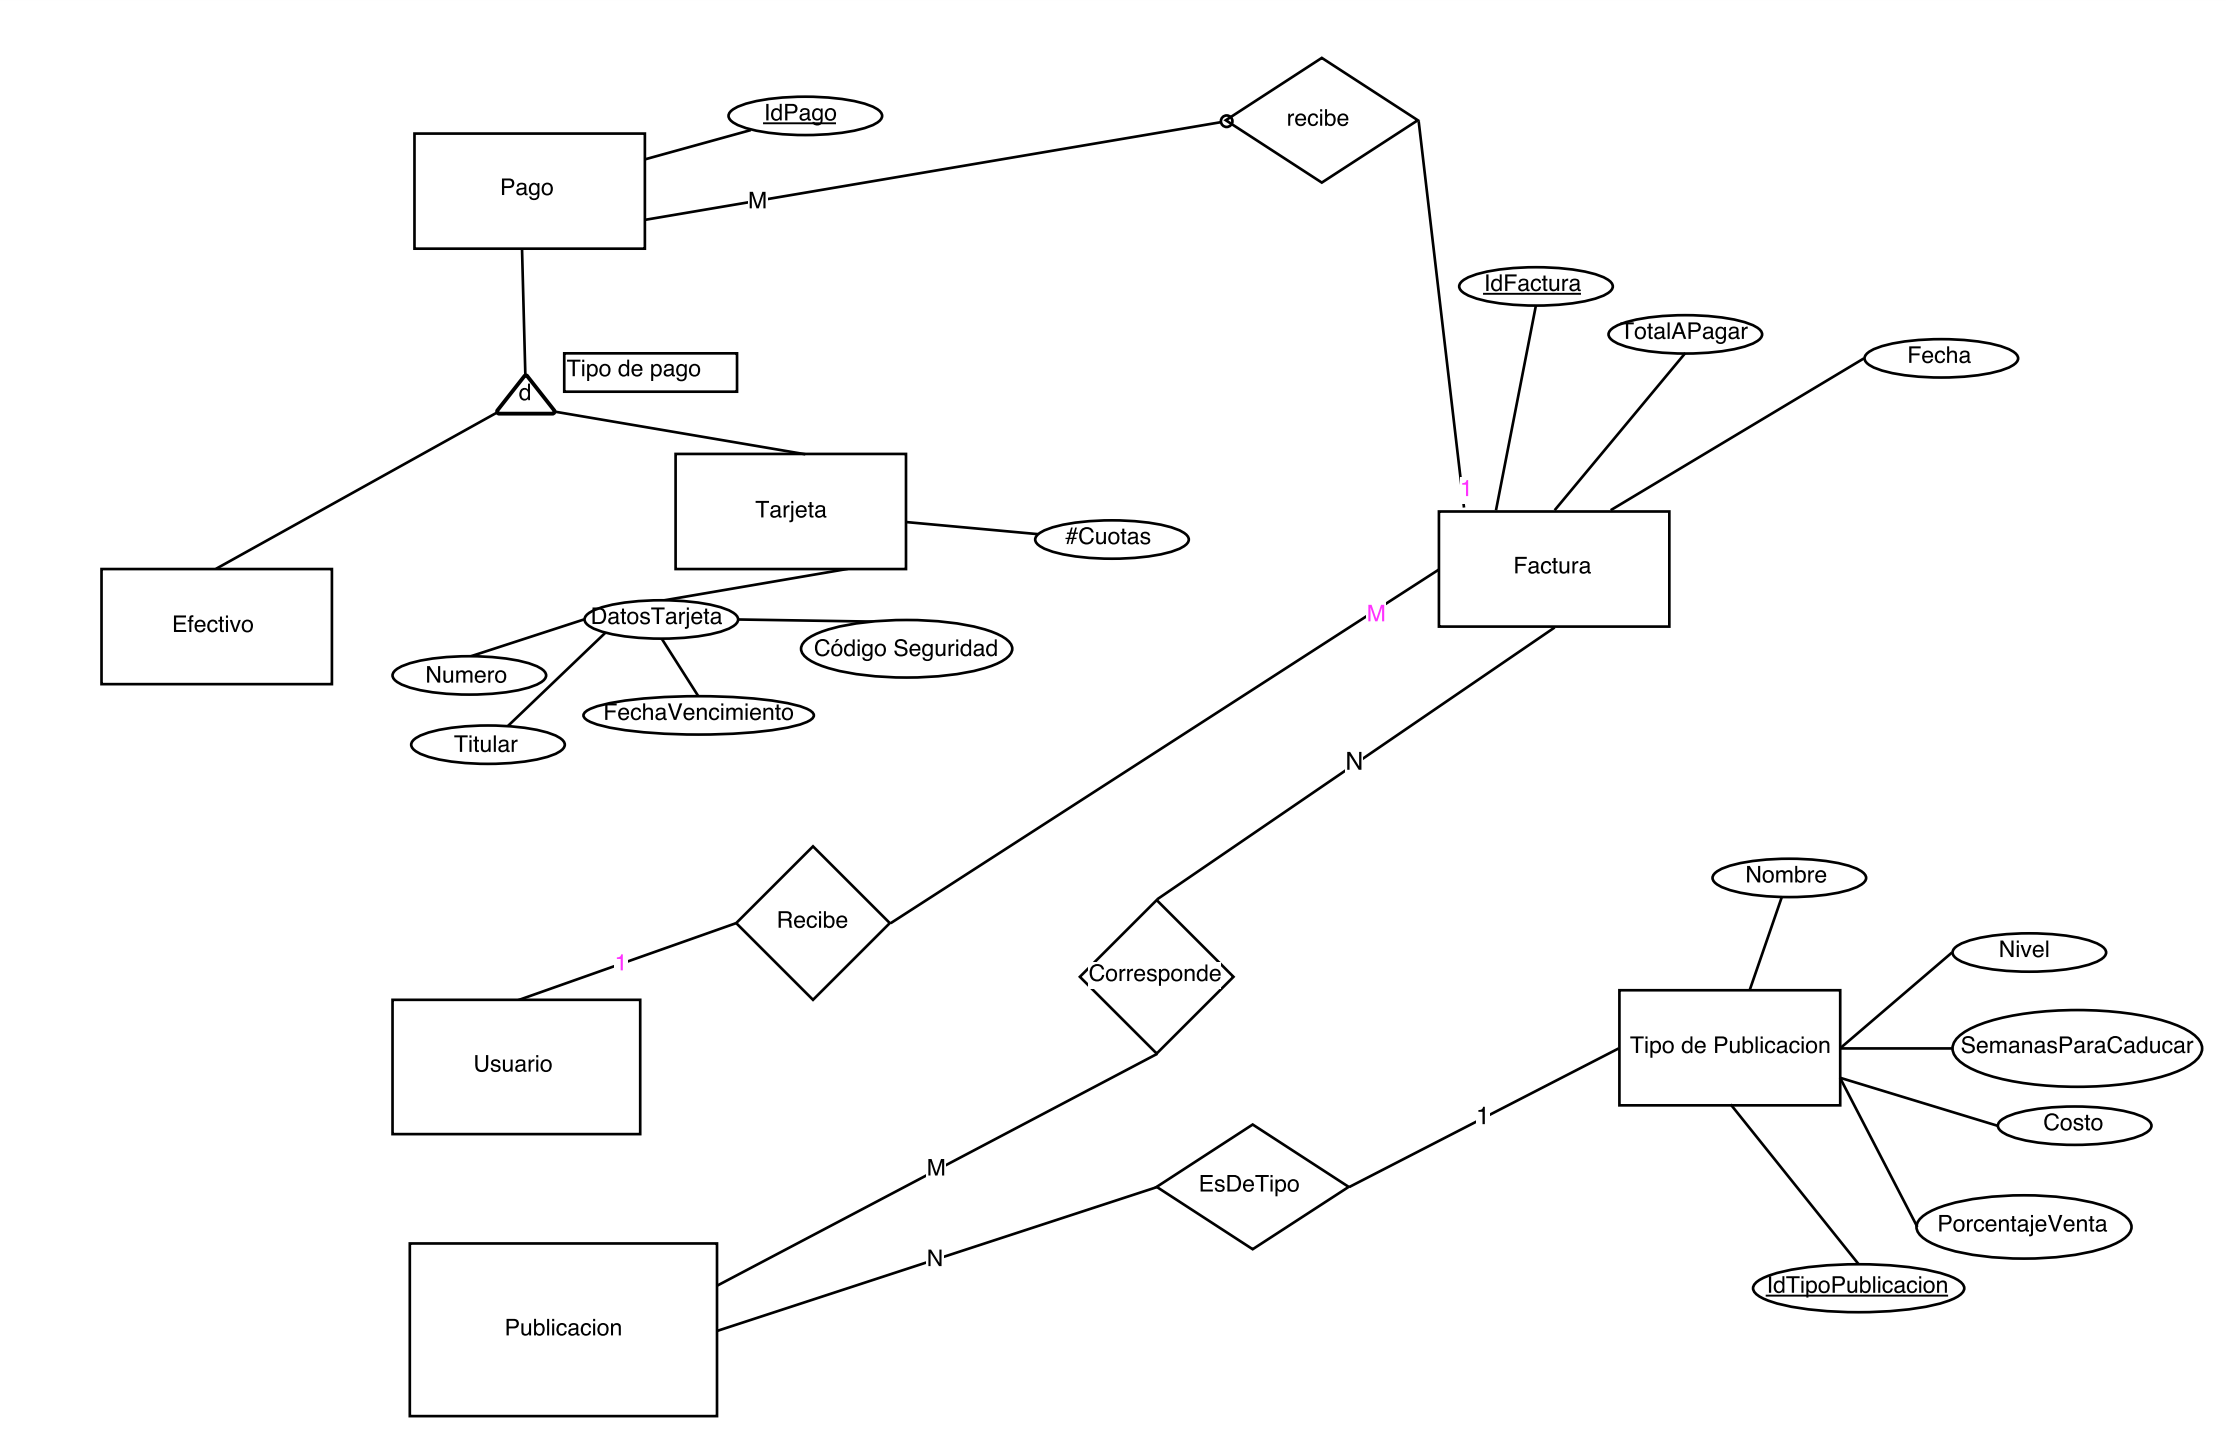
\includegraphics[width=18cm, height=12cm]{der3}
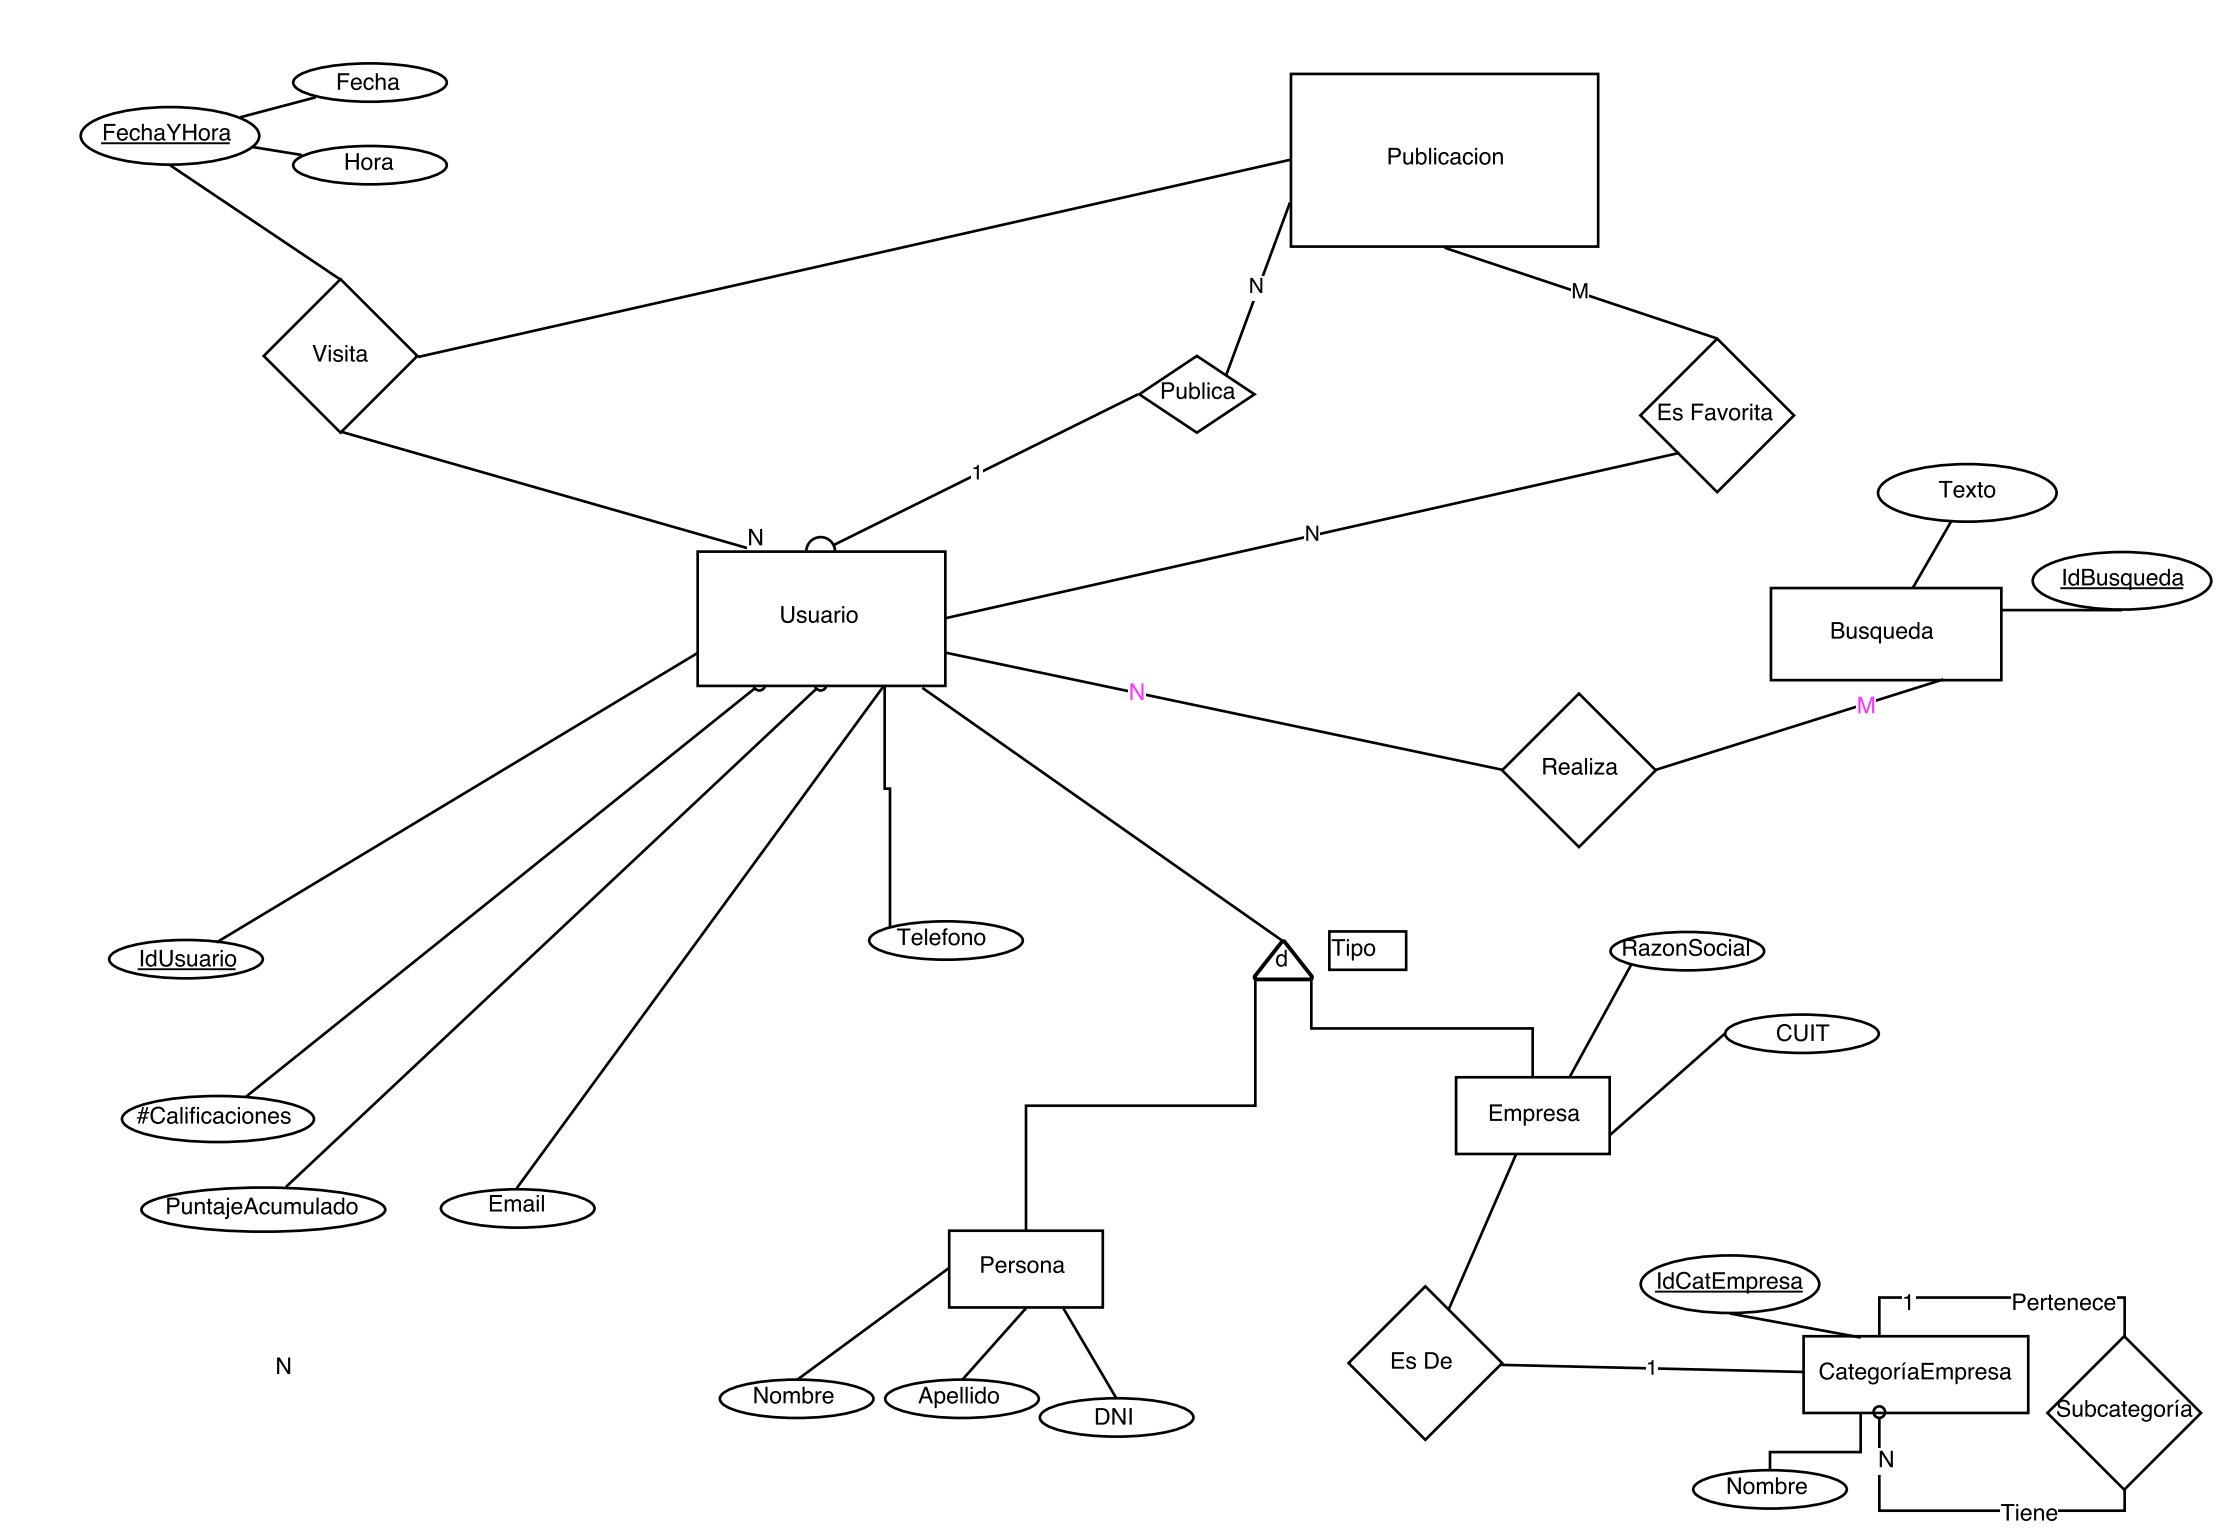
\includegraphics[width=18cm, height=12cm]{der4}
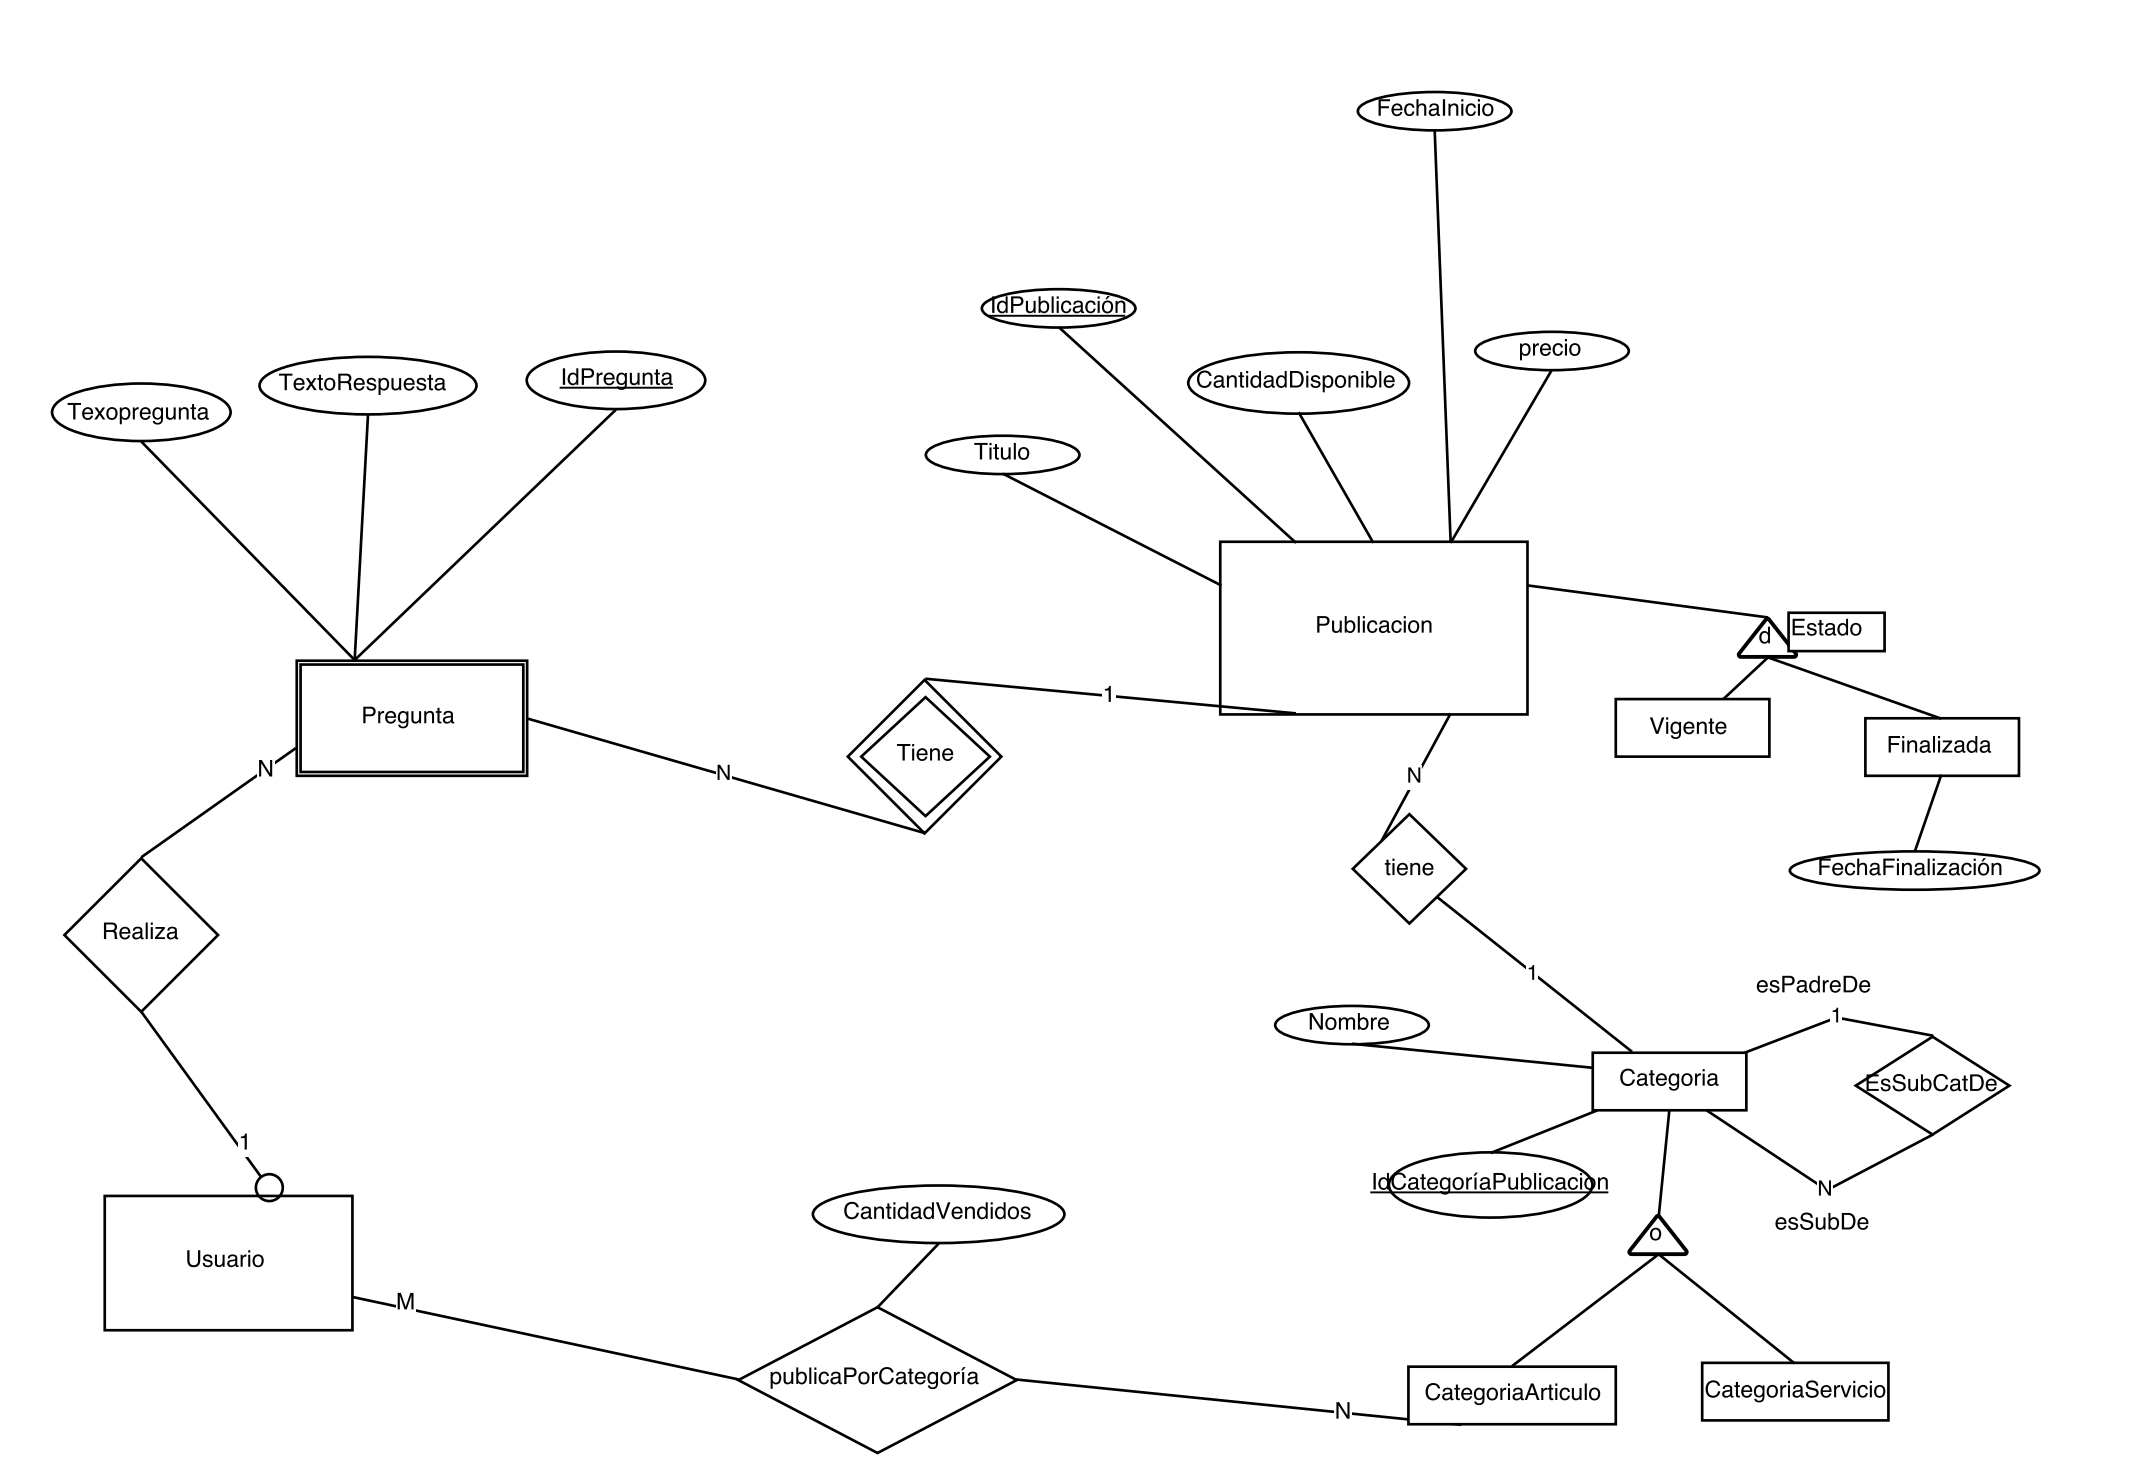
\includegraphics[width=19cm, height=12cm]{der5}

\subsection{Restricciones}




%%%%%%%%%%%%%%%%%%%%%%%%%%%%%%%%%%%%%%%%%%%%%%%%%%%%%%%%%%%%%%%%%%%%%%%%%%%%%%%
%% Modelo Relacional                                                         %%
%%%%%%%%%%%%%%%%%%%%%%%%%%%%%%%%%%%%%%%%%%%%%%%%%%%%%%%%%%%%%%%%%%%%%%%%%%%%%%%


\section{Modelo Relacional}


\relacion{Facultad}{
  \pk{idFacultad},
  nombre
}{
  \clavespkck{idFacultad}
}

\relacion{Empadronado}{
  \pk{DNI},
  nombre,
  fechaDeNacimiento,
  \fk{idFacultad},
  claustro
}{
  \clavespkck{DNI}
}

\relacion{Estudiante}{
  \pkfk{DNI},
  fechaDeInscripcion
}{
  \clavespkckfk{DNI}
}

\relacion{Graduado}{
  \pkfk{DNI},
  universidad
}{
  \clavespkckfk{DNI}
}

\section{Suposiciones}

\section{Diseno Fisico}

\section{Codigo}

\section{Conclusiones}


\end{document}
